% !Tex program = xelatex
\documentclass[a4paper,12pt]{article}

% -------------------- Packages --------------------
\usepackage[utf8]{inputenc}
\usepackage{graphicx}
\usepackage{amsmath,amssymb}
\usepackage{hyperref}
\usepackage{cite}

% 中文支持（如果需要） -> 使用 XeLaTeX 或 LuaLaTeX 编译
\usepackage{ctex}

% -------------------- Document Info --------------------
\title{论文标题示例}
\author{作者姓名}
\date{\today}

% -------------------- Document --------------------
\begin{document}


\maketitle

\begin{abstract}
这是摘要部分。
\end{abstract}

\section{引言}
这里是引言内容。引用示例文献~\cite{einstein1905}。

\section{相关工作}
这里是相关工作的内容。

\section{实验}
如图~\ref{fig:example} 所示。

\begin{figure}[h]
  \centering
  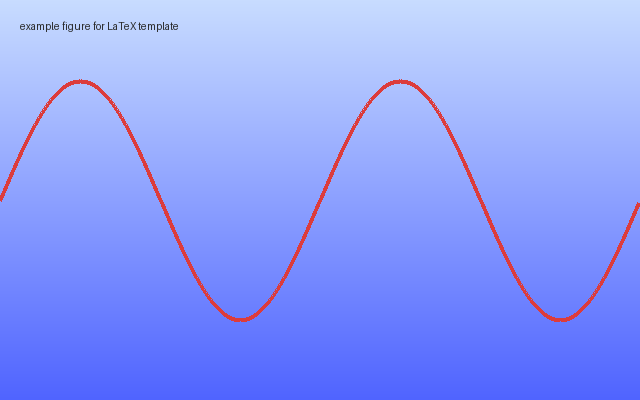
\includegraphics[width=0.5\textwidth]{figures/example.png}
  \caption{示例图片}
  \label{fig:example}
\end{figure}

\section{结论}
这里是结论。

\bibliographystyle{IEEEtran}
\bibliography{references}

\end{document}
